% \subsection{Implementing successive random additions (on a finite grid in 2 dimensions)}
\subsection{Implementation\label{subsec:SRA_implementation}}
In our implementation we generate a surface on a finite grid of size $N\times N$, starting with only the $z$-values in the four corners defined, giving a resolution $N_0 = 2$. As shown in \cref{eq:diamond_step_resolution} the algorithm can go from any resolution $N_0$ to any resolution $N_p = 2^p(n_0-1) + 1$ by applying the algorithm $p$ times, which means that our implementation can generate surfaces with resolutions
\begin{align*}
    N &= 2^p(2-1) + 1 = 2^p + 1,
\end{align*}
where $p$ is any positive integer.

We implement generation of both periodic and non-periodic surfaces using using \crefrange{eq:square_step_limits}{eq:diamond_step02}, while skipping points outside the grid for non-periodic surfaces, and wrapping around the edges using periodic boundary conditions when generating periodic surfaces.

To ensure that the periodic surfaces actually turn out periodic we start with all four corners having the same value. We also let the right and bottom edge be equivalent to the left and top edge, respectively, which effectively means that all four corners should always have the same $z$-value. To ensure that the opposite edges stay equal to each other we never generate any points on the right and bottom edge, but just copy the $z$-values from the opposite edge after the diamond-step.

This leaves us with the following algorithm for generating a surface which approximates a 2-dimensional fractional Brownian motion with Hurst exponent $H$
\begin{enumerate}
    % \itemsep1pt \parskip0pt \parsep0pt
    \renewcommand{\labelitemii}{$\bullet$}
    
    \item Allocate a grid of size $N\times N$, where $N = 2^p + 1$, and $p$ is any positive integer. This grid will store the $z$-values, or the height of the surface, in each grid point $z(x,y)$.

    \item Initialize the $z$-values of the corners of the grid by drawing random numbers from a Gaussian distribution with mean $\mu = 0$ and variance $\sigma_0$. The initial variance can be chosen freely. The initial resolution is now $2\times 2$.
    \begin{itemize}
        \item If generating a periodic surface, give all four corners the same $z$-value.
    \end{itemize}
    
    \item Apply the square-step using \cref{eq:square_step_limits,eq:square_step}. Add a random Gaussian number with mean $\mu = 0$ and variance $\sigma_n = \sigma_{n-1}^2r^{2H}$ to all new and old points.
    \label{enum:square_step}

    \item Apply the diamond-step using \crefrange{eq:diamond_step01}{eq:diamond_step02}. Add a random Gaussian number with mean $\mu = 0$ and variance $\sigma_{n+1} = \sigma_n^2r^{2H}$ to all new and old points.
    \label{enum:diamond_step}
    
    \begin{itemize}
        \item If generating a periodic surface, skip generating $z$-values for points on the right and bottom edge using the diamond-step, and instead copy the values from the opposite edges after the diamond-step.
    \end{itemize}
    
    \item Repeat step \ref{enum:square_step} and \ref{enum:diamond_step} $p$ times until you reach the desired resolution of $N\times N$, where $N = 2^p + 1$. For step $n$ the variance of the random Gaussian numbers is
    \begin{align*}
        \sigma_n^2 = \sigma_0^2(r^n)^{2H}.
    \end{align*}
\end{enumerate}

We implement the method in \cpp, and make a \matlab\ interface to the \cpp-program, for fast visualization and testing. We implement both generation of periodic and non-periodic surfaces, and the midpoint displacement method, and successive random additions. 

See \cref{fig:diamond_square_surface} for a surface with resolution $33\times 33$ generated by the algorithm.%
%
% \begin{figure}[htpb]%
%     \centering%
%     \includesvg[width=0.7\textwidth, svgpath=./images/diamond_square/surface_example/]{surface_labels}%
%     \caption{%
%         Caption.%
%         \label{fig:diamond_square_surface}%
%     }%
% \end{figure}%
\begin{figure}[htpb]%
    \centering%
    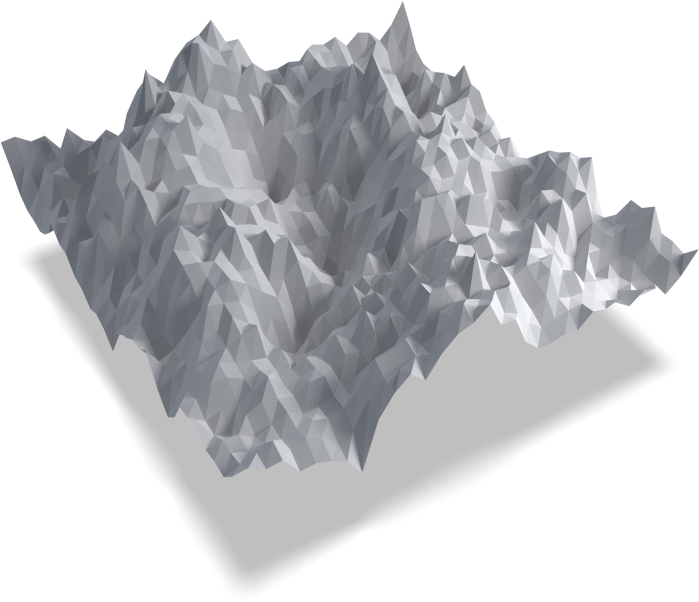
\includegraphics[width=0.5\textwidth]{./images/diamond_square/surface_blender/surface_composite01_cropped.png}%
    \caption{%
        A surface with resolution $33\times 33$ created using the midpoint displacement method called successive random additions.%
        \label{fig:diamond_square_surface}%
    }%
\end{figure}%
%
% \orangebox{
% {\bf Notes:}
% \begin{itemize}
%     \item Implementation (in Matlab/C++)?
%     \item periodic and non-periodic
%     \item Mention that DS can be used to increase resolution of any surface
%     \item Can increase resolution of generated surface, if we know the seed
% \end{itemize}
% 
% {\bf Stuff to define:}
% \begin{itemize}
%     \item Periodic/non-periodic
%     \item Lacunarity
% \end{itemize}
% }